%% Manuscript for Science of Computer Programming (Elsevier), research papers track.
%% Class: elsarticle (Elsevier's LaTeX class), submission mode (`review'). Numeric references.
%% Rules followed (SCP guide for authors, read 13 Nov 2026): abstract <= 250 words; 1-7 keywords;
%% highlights in a separate file (3-5 bullets, <= 85 characters); numbered sections; tables as editable
%% text without vertical rules; figures as separate files (figures/Figure_1.pdf, Figure_2.pdf);
%% CRediT, competing interests, funding, data availability and generative-AI statements before the references.
\documentclass[review,12pt]{elsarticle}

\usepackage{amssymb}
\usepackage{booktabs}
\usepackage{graphicx}
\usepackage{listings}
\usepackage{url}
\usepackage{lineno}
\modulolinenumbers[5]

\lstset{
  basicstyle=\ttfamily\footnotesize,
  columns=fullflexible,
  keepspaces=true,
  showstringspaces=false,
  frame=single,
  framerule=0.2pt,
  breaklines=true
}

\setlength{\emergencystretch}{3em}
\newcommand{\code}[1]{\texttt{#1}}
\newcommand{\crem}{\texttt{crem}}

\journal{Science of Computer Programming}

\begin{document}

\begin{frontmatter}

\title{Compile-time transition safety versus exhaustive testing in composable finite-state machines: an experimental comparison in Haskell, C and C++}

%% TODO(author): complete the postal address (the guide requires full name and postal address, with country),
%% the corresponding author's e-mail (it is published), and decide whether the advisor is a co-author.
\author[fatec]{Peterson Carara Junior\corref{cor1}}
\ead{[e-mail to be added]}
\cortext[cor1]{Corresponding author.}
\affiliation[fatec]{organization={Faculdade de Tecnologia da Baixada Santista ``Rubens Lara'' (Fatec BS)},
  addressline={[street and number to be added]},
  city={Santos},
  state={SP},
  country={Brazil}}

\begin{abstract}
Typed state-machine libraries promise that illegal transitions are rejected at compile time, while exhaustive testing over a finite domain is a common alternative. What does compile-time checking add? We implement one four-state machine in five ways (C with \code{enum} and \code{switch}; C++17 with \code{enum class}; C++17 with a type-level topology; Haskell with algebraic data types; Haskell with the \code{crem} library) and compare each with a transition table that records which rules come from the requirements and which are conventions. We inject defects from six classes and observe compiler diagnostics at three warning levels, a static analyser, a type checker and an exhaustive test of the 16 state--event pairs. A rejection matrix over all 16 vertex pairs is identical in \code{crem} and in C++17 with a type-level topology: the eight pairs outside the topology are rejected, each with the expected cause. Rejecting a forbidden transition at compile time is therefore not specific to Haskell. Omitted cases are stopped only when warnings are errors, and a catch-all clause hides them from default diagnostics. No compiler or analyser detected a wrong destination on an allowed edge; only the test did. Compiler output for an omitted case ranges from 4 to 236 lines. Compile-time checking advances detection and removes edge-specific tests, but does not make behavioural correctness equivalent to type safety. The study has one machine, one compiler per language and author-written code.
\end{abstract}

\begin{keyword}
finite-state machines \sep Haskell \sep type-level programming \sep static verification \sep mutation analysis \sep C++ \sep exhaustive testing
\end{keyword}

\end{frontmatter}

\linenumbers

\section{Introduction}
\label{sec:intro}

A finite-state machine is the standard model for reactive behaviour, and programming languages differ in how much of its specification they can check before the program runs. In C and in C++ with plain enumerations, states and events are integers in disguise, and a \code{switch} statement is the usual encoding; exhaustiveness is, at best, a compiler warning. In a pure functional language, states and events are algebraic data types and the compiler checks that the transition function covers every pair \cite{hutton2016haskell}. Libraries such as \crem{} \cite{perone2023crem} go further and lift the set of \emph{allowed transitions} (the topology) to the type level, so that an action returning a destination not permitted from its origin fails to type-check.

The usual argument for such a guarantee is that it moves the detection of a defect from testing to compilation. The argument is rarely tested against its natural alternative. In a finite domain, such as the 16 state--event pairs of a small machine, an exhaustive test is cheap to write, and other constructions, even in C++, may reject the same defects at compile time. This paper asks what compile-time checking adds, measured on a concrete machine.

\subsection{Research questions}
\label{sec:rqs}

\begin{description}
\item[RQ1] Which classes of defect does each mechanism (compiler warnings at several levels, a static analyser, a type checker, an exhaustive test) detect, in each of five implementations?
\item[RQ2] Is the compile-time rejection of a forbidden transition specific to Haskell and \crem{}?
\item[RQ3] What does an exhaustive test add to compile-time checking, and what can it not see?
\item[RQ4] What does the diagnostic cost, measured as the size of the compiler output?
\end{description}

\subsection{Contributions}
\label{sec:contrib}

\begin{enumerate}
\item A controlled comparison of five implementations of the same machine against one transition table, with six defect classes and four mechanisms, reproducible with a single script (Sect.~\ref{sec:design}).
\item A matrix of all 16 ordered vertex pairs, with the cause of each rejection checked, for \crem{} and for a C++17 construction with a type-level topology: the outcomes are identical (Sect.~\ref{sec:matrix}).
\item The observation that the gap between ``warns'' and ``rejects'' for omitted cases is a configuration, not a language, difference, and that a catch-all clause hides omissions from the default diagnostics of all five stacks (Sect.~\ref{sec:classes}).
\item The observation that no compiler or analyser in the study detects a wrong destination on an allowed edge, so the guarantee of a type-level topology is per edge and not per event (Sect.~\ref{sec:classes}).
\item A measurement of the size of the diagnostics, which differs by two orders of magnitude between constructions (Sect.~\ref{sec:diag}).
\end{enumerate}

\subsection{Scope}
\label{sec:scope}

The subject is a four-state machine used as an illustration; there are no safety requirements behind it, and nothing is claimed about real avionics. The paper proposes no new type system and no formal semantics. The behaviour of this machine when composed with others and fed back is the subject of a companion manuscript in preparation; the results reported here do not depend on it.

\section{Background}
\label{sec:background}

\subsection{Typed topologies in crem}

A \crem{} machine is a Mealy machine: it emits an output and updates its state on each input. Its vertices are promoted to the type level with the \code{singletons} library \cite{eisenberg2012singletons}, and the \emph{topology} is a value listing, for each vertex, the vertices that may follow it. The action receives the current vertex as a singleton and builds its result with \code{pureResult}, which requires the constraint \code{AllowedTransition} for the pair (origin, destination); the identity edge is always allowed. In \code{crem} 0.1.0.0 this constraint is solved by four instances marked \code{INCOHERENT} (we read the source of the package), so resolution is a search for any proof, and a missing edge leaves an unsolved constraint. A transition whose destination is not in the topology of its origin is a compile-time error. The topology is not tied to the input that triggers a transition; this is acknowledged as a limitation by the authors of the library \cite{perone2023crem}. The idea that types change with protocol state, and that illegal operation sequences can be detected at compile time, is much older \cite{strom1986typestate}.

\subsection{Imperative encodings and compiler diagnostics}

In C, the usual encoding is an \code{enum} for states, another for events, and nested \code{switch} statements. A \code{switch} over an enumeration without a \code{default} makes the compiler warn about an unhandled enumerator (\code{-Wswitch}); with a \code{default} the warning disappears unless a stricter flag (\code{-Wswitch-enum}) is used. The two enumerations are interchangeable integers in C, so comparing a state with an event compiles. C++11 \code{enum class} types are distinct and not implicitly convertible \cite{iso14882}. In C++17, \code{std::variant} and \code{std::visit} require a callable for every combination of alternatives, and templates with \code{static\_assert} can encode a topology in types \cite{iso14882}. Clang \cite{clang} offers warning flags and a static analyser \cite{clanganalyzer}; GHC \cite{ghc} reports incomplete patterns as a warning (\code{-Wincomplete-patterns}) that a project may promote to an error.

\subsection{Mutation analysis}

To learn what a mechanism can detect, we inject defects into a correct program and observe whether the mechanism notices. This is the idea of mutation analysis \cite{demillo1978hints,jia2011mutation}. Our mutants are deliberate, one per class, and are not a sample of real faults.

\section{Study design}
\label{sec:design}

Figure~\ref{fig:design} shows the design.

\begin{figure}[t]
\centering
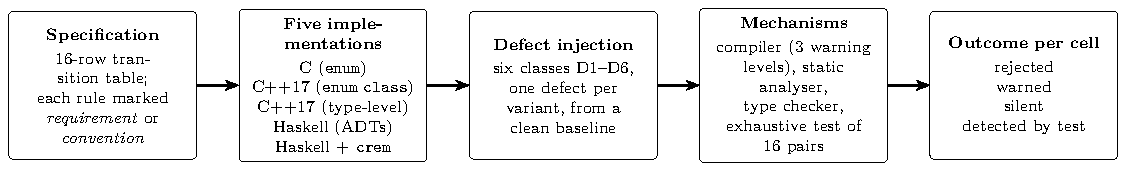
\includegraphics[width=\textwidth]{figures/Figure_1.pdf}
\caption{Study design. One transition table is the reference for five implementations, each with a clean baseline and one injected defect per variant; each variant is observed through several mechanisms.}
\label{fig:design}
\end{figure}

\subsection{Subject machine and specification}
\label{sec:spec}

The machine has four states (\code{Grounded}, \code{InFlight}, \code{EmergencyLanding}, \code{Shutdown}) and four events (\code{TakeoffSignal}, \code{CriticalBattery}, \code{LandedSignal}, \code{SystemCutoff}); each event also produces an output message. The specification is a table of 16 rows, one per (state, event) pair, written from the requirement text. Only four rows are stated there (Table~\ref{tab:delta}); the other twelve pairs are a project convention (the state does not change), and the output names are also a convention. The table records the origin of each row so that a reviewer can see what is assumed. The one prohibition in the requirements is the direct edge from \code{InFlight} to \code{Shutdown}. All implementations are compared with this table.

\begin{table}[t]
\caption{Destination of each (state, event) pair. \texttt{R}: stated in the requirement text. Unmarked cells keep the state (project convention).}
\label{tab:delta}
\centering
\scriptsize
\setlength{\tabcolsep}{3pt}
\begin{tabular}{@{}lllll@{}}
\toprule
State & \code{TakeoffSignal} & \code{CriticalBattery} & \code{LandedSignal} & \code{SystemCutoff} \\
\midrule
\code{Grounded}         & \code{InFlight} (R) & -- & -- & \code{Shutdown} (R) \\
\code{InFlight}         & -- & \code{EmergencyLanding} (R) & -- & -- \\
\code{EmergencyLanding} & -- & -- & \code{Grounded} (R) & -- \\
\code{Shutdown}         & -- & -- & -- & -- \\
\bottomrule
\end{tabular}
\end{table}

\subsection{Implementations}

Five implementations realise the table (Table~\ref{tab:stacks}). Each prints its 16 triples (state, event, destination) so that it can be compared with the table.

\begin{table}[t]
\caption{The five implementations and the toolchain used.}
\label{tab:stacks}
\centering
\footnotesize
\begin{tabular}{@{}p{2.1cm}p{4.2cm}p{5.8cm}@{}}
\toprule
Stack & Encoding & Toolchain \\
\midrule
C & \code{enum} and nested \code{switch} & clang 14.0.6, default C standard \\
C++ & \code{enum class} and nested \code{switch} & clang++ 14.0.6, \code{-std=c++17} \\
C++17 typed & \code{std::variant} states and events; a trait \code{Allowed} and \code{static\_assert} encode the topology; \code{std::visit} dispatches & clang++ 14.0.6, \code{-std=c++17} \\
Haskell & algebraic data types, one equation per pair, no wildcard & GHC 9.6.7 \\
Haskell + \crem{} & singleton vertices, type-level topology, \code{pureResult} & GHC 9.6.7, \code{crem} 0.1.0.0, with \code{-Werror=incomplete-patterns} \\
\bottomrule
\end{tabular}
\end{table}

The C++17 typed implementation is our own construction: a primary template \code{Allowed<From, To>} that is true only for identity, specialisations for the four edges, and a function \code{go<To>(from)} whose \code{static\_assert} fails when the pair is not allowed. It needs about ten lines beyond the transition function. It is not a recommendation of style; it tests the boundary of the claim that only Haskell can do this.

\subsection{Defect classes}

Table~\ref{tab:classes} lists the six defect classes. Each variant contains exactly one defect.

\begin{table}[t]
\caption{Defect classes. The example is the concrete defect injected in the C-family stacks; the same class is instantiated analogously in the others.}
\label{tab:classes}
\centering
\footnotesize
\begin{tabular}{@{}lp{3.4cm}p{6.6cm}@{}}
\toprule
Id & Class & Example \\
\midrule
D1 & omitted pair, no catch-all & the (\code{InFlight}, \code{LandedSignal}) case removed \\
D2 & omitted pair with a catch-all & the same case removed and a \code{default} (or a final wildcard clause) added \\
D3 & forbidden transition & (\code{InFlight}, \code{SystemCutoff}) goes to \code{Shutdown} \\
D4 & wrong destination on an allowed edge & (\code{Grounded}, \code{TakeoffSignal}) goes to \code{Shutdown}, an edge that exists from \code{Grounded} \\
D5 & state and event confused & a state is compared with an event constant, or an event is used as a destination \\
D6 & value outside the enumeration & the integer 42 returned as a state \\
\bottomrule
\end{tabular}
\end{table}

\subsection{Mechanisms}

\begin{itemize}
\item \textbf{Compiler, three levels (C-family).} A: \code{-Wall -Wextra}. B: A plus \code{-Wswitch-enum -Wenum-compare -Wassign-enum}. W: B plus \code{-Werror}, the analogue of promoting incomplete patterns to errors in Haskell.
\item \textbf{Static analyser.} \code{clang --analyze}.
\item \textbf{Type checker.} The Haskell and C++17 typed outcomes, including the type-level topology.
\item \textbf{Exhaustive test.} A harness that prints the 16 triples and compares them with the table. For \crem{}, the equivalent is a suite that compares the action's destination and output for every pair with the table.
\end{itemize}

For Haskell the compiler levels are \code{-Wall} and \code{-Wall} with \code{-Werror=incomplete-}\allowbreak\code{patterns}. For \crem{} we also injected nine defects into the real library code (Sect.~\ref{sec:crem}).

\subsection{Procedure and reproducibility}

Every outcome in this paper comes from scripts that generate the variants by editing the clean baselines, compile them, run the harness and write the results. The baselines print the table exactly (no warning in any mechanism). Versions: clang 14.0.6 (the one shipped with GHC), GHC 9.6.7, \code{crem} 0.1.0.0, Windows 11. The scripts, tables and logs are part of the artefact (see the data availability statement).

\section{Results}
\label{sec:results}

\subsection{Rejecting forbidden transitions: crem and C++17 give the same matrix}
\label{sec:matrix}

For each of the 16 ordered pairs of vertices we generate a minimal program that requests the transition and compile it. The expected outcome comes from the table: the four edges and the four identities compile, the other eight pairs must be rejected. A pair counts as rejected only if the compiler reports exactly one error and the error names the pair (for \crem{}, \code{Could not deduce AllowedTransition} for the pair; for C++17, a failed \code{static\_assert} naming \code{Allowed<From, To>}). All 16 results agree with the table in both stacks, and the two matrices are identical (Table~\ref{tab:matrix}).

\begin{table}[t]
\caption{Compilation of a request for each (origin, destination) pair; identical in \crem{} and in C++17 with a type-level topology. $\checkmark$: compiles (identity on the diagonal); $\times$: rejected with the expected cause.}
\label{tab:matrix}
\centering
\footnotesize
\begin{tabular}{@{}lcccc@{}}
\toprule
origin $\backslash$ destination & \code{Grounded} & \code{InFlight} & \code{EmergencyLanding} & \code{Shutdown} \\
\midrule
\code{Grounded}         & $\checkmark$ & $\checkmark$ & $\times$ & $\checkmark$ \\
\code{InFlight}         & $\times$ & $\checkmark$ & $\checkmark$ & $\times$ \\
\code{EmergencyLanding} & $\checkmark$ & $\times$ & $\checkmark$ & $\times$ \\
\code{Shutdown}         & $\times$ & $\times$ & $\times$ & $\checkmark$ \\
\bottomrule
\end{tabular}
\end{table}

The answer to RQ2 is therefore no: a forbidden transition can be rejected at compile time without Haskell, with a small amount of template machinery. The matrix checks the \emph{topology}; it is not the same as the state-by-event matrix, which also has 16 cells but concerns the coverage of the transition function and is the subject of D1 and D2.

\subsection{Defect classes and mechanisms}
\label{sec:classes}

Table~\ref{tab:results} summarises what each mechanism does with each defect class in each stack.

\begin{table}[!t]
\caption{Outcome per defect class and stack. ``Error'' = the compiler or type checker rejects; ``warning'' = compiles with a warning; ``silent'' = compiles without a diagnostic; ``test'' = the exhaustive test result. $^{a}$ the omitted pair's fallback equals the specified behaviour (identity), so the test passes. $^{b}$ variant H9, which omits a pair whose specified behaviour is not the identity; the compiler is equally silent and the test fails.}
\label{tab:results}
\centering
\scriptsize
\begin{tabular}{@{}p{1.0cm}p{2.0cm}p{2.0cm}p{2.0cm}p{2.0cm}p{2.0cm}@{}}
\toprule
Class & C & C++ & C++17 typed & Haskell & Haskell + \crem{} \\
\midrule
D1 & warning (A, B); error with W. Test$^{a}$ passes & warning (A, B); error with W. Test$^{a}$ passes & error (no matching function) & warning; error with \code{-Werror=} \code{incomplete-} \code{patterns}; test: run-time exception & error (exhaustiveness as error) \\
D2 & silent in A; warning in B; error with W. Test$^{a}$ passes & silent in A; warning in B; error with W. Test$^{a}$ passes & silent. Test$^{a}$ passes & silent. Test$^{a}$ passes & silent$^{b}$; test fails$^{b}$ \\
D3 & silent; test detects & silent; test detects & error (\code{static\_assert}) & silent; test detects & error (no proof of the edge) \\
D4 & silent; test detects & silent; test detects & silent; test detects & silent; test detects & silent; test detects \\
D5 & silent; test detects only by numeric coincidence & error (distinct types) & error & error (type mismatch) & error (type mismatch) \\
D6 & silent; test detects & silent (\code{static\_cast}); test detects & not applicable (closed sum) & error (no \code{Num} instance) & error \\
\bottomrule
\end{tabular}
\end{table}

\paragraph{D1 and D2: omitted cases} In C and C++, an omitted case in a \code{switch} without \code{default} is a warning already at level A (the warning is part of \code{-Wall}); with a \code{default}, the warning appears only at level B; and with \code{-Werror} (level W) both become errors. In Haskell the incomplete-patterns warning is part of \code{-Wall} and becomes an error with a flag that the \crem{} project sets. In C++17 with \code{std::visit}, an omitted pair is an error because the visitor has no overload for that combination. A catch-all clause hides the omission from the default diagnostics of every stack. Only C and C++ have a stricter flag, \code{-Wswitch-enum}, that exposes it (levels B and W), at the price of also flagging legitimate \code{default} clauses; in C++17 typed, Haskell and \crem{} nothing in our configurations flags it. The difference between ``warns'' and ``rejects'' is a matter of configuration, not of language.

In the \crem{} variant of D2 (H9), the actions for \code{Grounded} with \code{TakeoffSignal} were removed and a final clause \code{avionicsAction s \_ = pureResult MsgIgnored s} (an identity, which is always an allowed edge) was added: the library compiles without a diagnostic, and the behaviour changes. In the variants of the other stacks, the omitted pair happened to be one whose specified behaviour is the identity, so the test passes while the compiler's silence or warning is the only signal. We return to this asymmetry in Sect.~\ref{sec:test}.

\paragraph{D3: forbidden transition} It is invisible to the C and C++ compilers and analyser and to plain Haskell, and is detected by the exhaustive test. It is rejected at compile time by the C++17 typed construction and by \crem{}. This is the class where the type-level topology adds something, and it adds the same in the two stacks that have it.

\paragraph{D4: wrong destination on an allowed edge} Every stack is silent at compile time, and only the test detects it. The reason is structural: the topology fixes which vertices may follow which, not which event leads to which vertex. In the C++17 typed variant, redirecting the take-off from \code{InFlight} to \code{Shutdown} still satisfies \code{Allowed<Grounded, Shutdown>}. No compiler or analyser in the study detected this class.

\paragraph{D5 and D6} Distinct types for states and events turn the confusion of D5 into an error in every stack except C, where the two enumerations convert to each other; the test detects it only because the numeric values of the two constants happen to differ for the compared pair. An out-of-range value (D6) is an error in Haskell, impossible by construction in the C++17 typed variant (a variant of unrelated types has no such value), and silent in C and C++ (a \code{static\_cast} suffices).

\paragraph{Static analyser} \code{clang --analyze} reported nothing for any variant that compiles. This holds for this analyser and version with its default checks, and says nothing about static analysis in general.

\subsection{The Haskell library code under mutation}
\label{sec:crem}

To see whether the pattern holds in real library code, we injected nine defects, one at a time, into the \crem{} implementation of the machine and of the components around it (the battery machine and an environment machine of a larger system), and ran five test suites on each. Two defects were rejected by the compiler: an illegal edge in the action without a change to the topology, and an omitted pair. Seven were accepted and killed by at least one suite: an illegal edge added to both topology and action, a wrong destination on an allowed edge, swapped events, a wrong output, two defects in the components around the machine, and the catch-all variant above. No mutant survived. The full list of mutants is in the artefact. Compile-time rejection covered two of nine defects; the remaining seven were found by tests, among them those of D4 and of the output of an action, which the type does not mention.

\subsection{Size of the diagnostics}
\label{sec:diag}

Figure~\ref{fig:diag} shows the size, in lines, of the compiler output for six rejected or warned defects. The \code{-Wswitch} warning of C and the type mismatch of C++ \code{enum class} have 4 lines; the \code{static\_assert} that rejects a forbidden transition in C++17 has 7; the \crem{} error for the same defect has 25 lines (1\,637 bytes); and an omitted case in \code{std::visit} has 236 lines (35\,863 bytes) of template instantiation messages. Size is not readability: there was no reader study. It is an upper bound on what the engineer must scan to find the cause.

\begin{figure}[t]
\centering
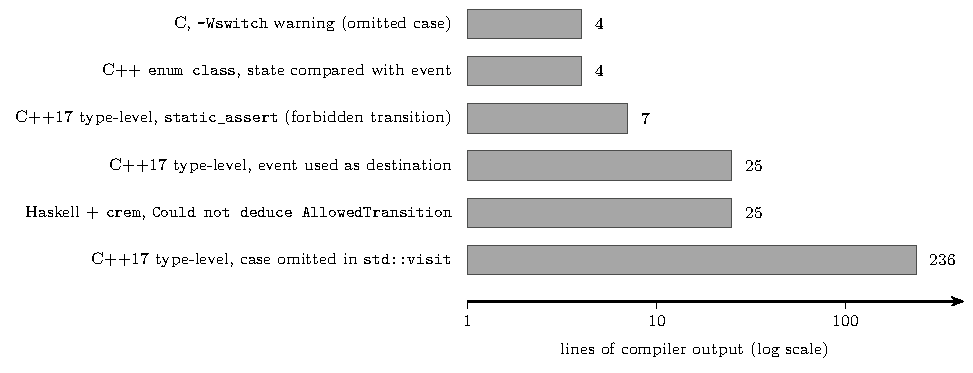
\includegraphics[width=0.95\textwidth]{figures/Figure_2.pdf}
\caption{Size of the compiler output for six defects (logarithmic scale).}
\label{fig:diag}
\end{figure}

\subsection{What the exhaustive test adds, and what it cannot see}
\label{sec:test}

Over a finite domain of 16 pairs, the exhaustive test detected every defect that changes the behaviour in every stack in which it compiles (D3, D4, D5 and D6 in C; D3, D4 and D6 in C++; D4 in C++17 typed; D1, D3 and D4 in plain Haskell, where D1 appears as a run-time exception; and all \crem{} mutants that compile). It cannot see a latent defect whose consequence equals the specified behaviour: an omitted pair whose fallback is the identity passes the test (D1 and D2 in C and C++; D2 in C++17 typed and in Haskell). That is exactly the class that compilers flag when warnings are errors. The two mechanisms are complementary: the test catches what changes behaviour, the strict compiler what \emph{would} change it if the specification changed. Note that the test must include the \emph{events}: a test of the topology alone, such as the matrix of Sect.~\ref{sec:matrix}, cannot detect D4.

\section{Discussion}
\label{sec:discussion}

\paragraph{What compile-time checking buys} In this study, compile-time checking advanced the detection of two classes: omitted cases (when warnings are errors) and forbidden transitions (when the topology is in the types). For those classes it also removes the need to write a test: the edge-specific tests for D3 are unnecessary where the type-level topology exists. This is a real gain in the position and cost of detection. It is not a gain in coverage: the exhaustive test detected the same behavioural defects.

\paragraph{It is not specific to Haskell} A construction in C++17 of about ten lines reproduces the 16-pair rejection matrix of \crem{}. The cost is in the diagnostics (up to 236 lines for an omitted pair) and in the constructs the programmer must know. The claim that Haskell detects defects that C or C++ cannot would be too broad; what is verifiable is that certain topology constraints are checked at compile time in \crem{}, which anticipates their detection and dispenses with specific tests for those edges.

\paragraph{The event--destination gap is shared} The one class that no compiler or analyser detected, D4, is the one that matters for behaviour: the wrong consequence of an event on an allowed edge. Tying events to edges in the types is possible in principle with indexed monads \cite{atkey2009parameterised} or dependently typed languages \cite{brady2013idris}; none of the stacks here does it, and we did not evaluate these alternatives. With the tools as they are, the defence is a specification that includes events, checked by an exhaustive test.

\paragraph{Practical recommendations, within this study} (i) Compile with warnings as errors, and in particular promote exhaustiveness to an error. (ii) Avoid catch-all clauses in transition functions, or review them as part of the specification. (iii) Test the events, not only the edges. (iv) If a type-level topology is wanted, a library is not the only way.

\subsection{Threats to validity}
\label{sec:threats}

\paragraph{One machine} The subject has four states and four events. Larger machines and other topologies may change the cost, but the structure of the classes does not depend on size; the cost of diagnostics and of compilation does, and we did not measure compilation time.

\paragraph{Authorship and review} The same person wrote the five implementations, the table, the defects and the scripts. The C and C++ code, in particular, was written by an author with little experience in those languages, and has not been reviewed by an independent C or C++ expert; the typed C++17 construction is one possible design among others (for instance \code{constexpr} tables or C++20 concepts). A review is pending. The defects are deliberate and are not a sample of real faults.

\paragraph{One compiler per language} We used clang 14.0.6 for C and C++ and GHC 9.6.7 for Haskell, on one operating system. GCC, MSVC and other analysers may behave differently; \code{clang-tidy} was not available in the toolchain used.

\paragraph{Proxies} The size of the diagnostics is a proxy for readability; maintenance effort was not measured.

\paragraph{Procedure} The scripts and a first draft of this text were produced with the assistance of a generative AI system (see the statement before the references). Every figure of the paper comes from a recorded run, and the scripts check that the clean baselines print the table exactly, so that the variants differ from a verified baseline by one defect.

\section{Related work}
\label{sec:related}

This section is not a systematic review; a protocol for one exists in the artefact but the search has not been carried out, and the paper does not claim novelty beyond what is stated in Sect.~\ref{sec:contrib}.

Typed encodings of state machines in Haskell are the subject of \crem{} \cite{perone2023crem}, which builds on singletons \cite{eisenberg2012singletons}, and of indexed monads \cite{atkey2009parameterised}. Typestate \cite{strom1986typestate} is the classic formulation of protocol-dependent types. The comparison of finite-state machines in imperative and in pure functional languages was also treated in Russian-language work \cite{malakhovski2009fsm}, which we cite only for the general observation that imperative encodings use enumerations and a mutable state variable. Mutation analysis \cite{demillo1978hints,jia2011mutation} is the basis of our defect injection. What we add is a controlled comparison of concrete mechanisms across five implementations of the same machine, including a C++17 construction that matches a type-level library on the topology matrix.

\section{Conclusions}
\label{sec:conclusions}

For a four-state machine, a type-level topology rejects exactly the eight vertex pairs outside the topology, both in \crem{} and in a C++17 construction of about ten lines. Rejecting a forbidden transition at compile time is not specific to Haskell. Omitted cases are stopped only when warnings are errors, and a catch-all clause hides them from the default diagnostics of every stack. The class that matters for behaviour, a wrong destination on an allowed edge, was detected by no compiler or analyser and by every exhaustive test. Compile-time checking anticipates detection and removes edge-specific tests; it does not make behavioural correctness equivalent to type safety. Future work includes other machines and scales, an independent review of the C and C++ code, other compilers and analysers, and a study of maintenance effort.

\section*{CRediT authorship contribution statement}
\textbf{[To be completed by the authors, using the CRediT roles required by the journal (e.g. Conceptualization, Methodology, Software, Investigation, Writing -- original draft, Supervision).]}

\section*{Declaration of competing interest}
\textbf{[To be completed by the authors.]}

\section*{Funding}
\textbf{[To be completed by the authors: list the funding sources, or, if there were none, state that this research did not receive any specific grant from funding agencies in the public, commercial, or not-for-profit sectors.]}

\section*{Data availability}
The scripts, the transition table, the C, C++ and Haskell sources, the generated variants and all logs are in the artefact of this work: a frozen snapshot of the \code{avionics-crem} repository (commit \code{9689ce8}) and the added folders with the experiment scripts. \textbf{[Public repository URL and archived DOI to be added before submission; the repository was private at the time of writing.]} One script rebuilds and reruns everything.

\section*{Declaration of generative AI and AI-assisted technologies in the manuscript preparation process}
During the preparation of this work the author used Claude (Anthropic), through Claude Code, to write the experiment scripts and a first draft of this text, and to run the experiments whose results are reported. \textbf{[The author to confirm: ``After using this tool, the author reviewed and edited the content as needed and takes full responsibility for the content of the published article'', and to state the extent of the review.]}

\bibliographystyle{elsarticle-num}
\bibliography{refs}

\end{document}
